\section{Robotermanipulation}
\subsection{Definition}
\begin{minipage}[t]{0.5\linewidth}
    \textbf{Effektor}\newline
    ist Teil des Handhabungsgeräts. Er wird am Handgelenk befestigt und an Energie und Steuerleitungen angeschlossen.
\end{minipage}
\begin{minipage}[t]{0.5\linewidth}
    \textbf{Greifer}\newline
    Ein Greifer ist das jenige Subsystem eines Industrieroboters, das eine 
    begrenzte Anzahl von geometrisch bestimmten Werkstücken für einen 
    bestimmten Zeitraum hält, d.h. die Position und Orientierung dieser 
    Werkstücke relativ zum Werkzeug-Koordinatensystem sichert.
\end{minipage}
\subsection{Hauptfunktion Greifer}
\begin{minipage}{0.5\linewidth}
\begin{itemize}
    \item Vorbereiten eines Kontakts
    \begin{itemize}
        \item bekannte Objektpositon und Orientirung erreichen
    \end{itemize}
    \item Herstellung des Kontakts zwischen Objekt und Greiffinger
    \item Manipulation des Objekts mit dem Greifer
        \begin{itemize}
        \item Ortsveränderung, Drehung, Montieren
    \end{itemize}
    \item Ablegen des Greifobjekts durch lösen des Kontakts
\end{itemize}
\end{minipage}
\begin{minipage}{0.5\linewidth}
    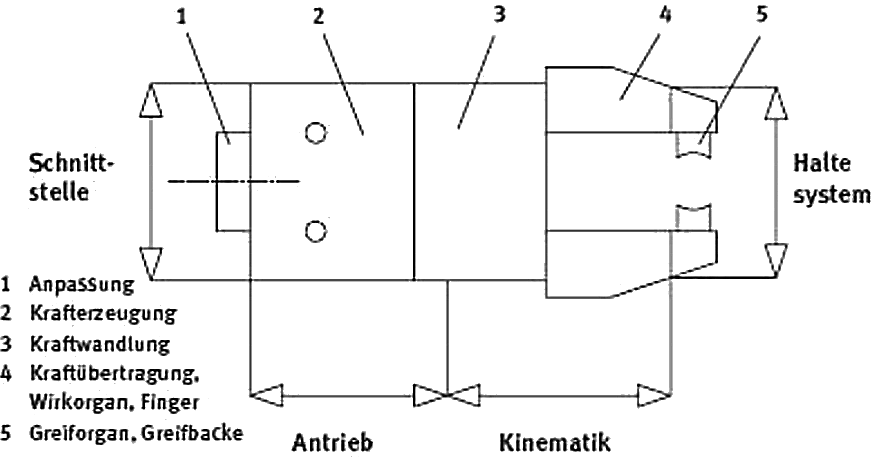
\includegraphics[width=\linewidth]{./bilder/Greifer}
\end{minipage}
\begin{minipage}{\linewidth}
    \subsection{Lösungsfindung für den Greifer}
    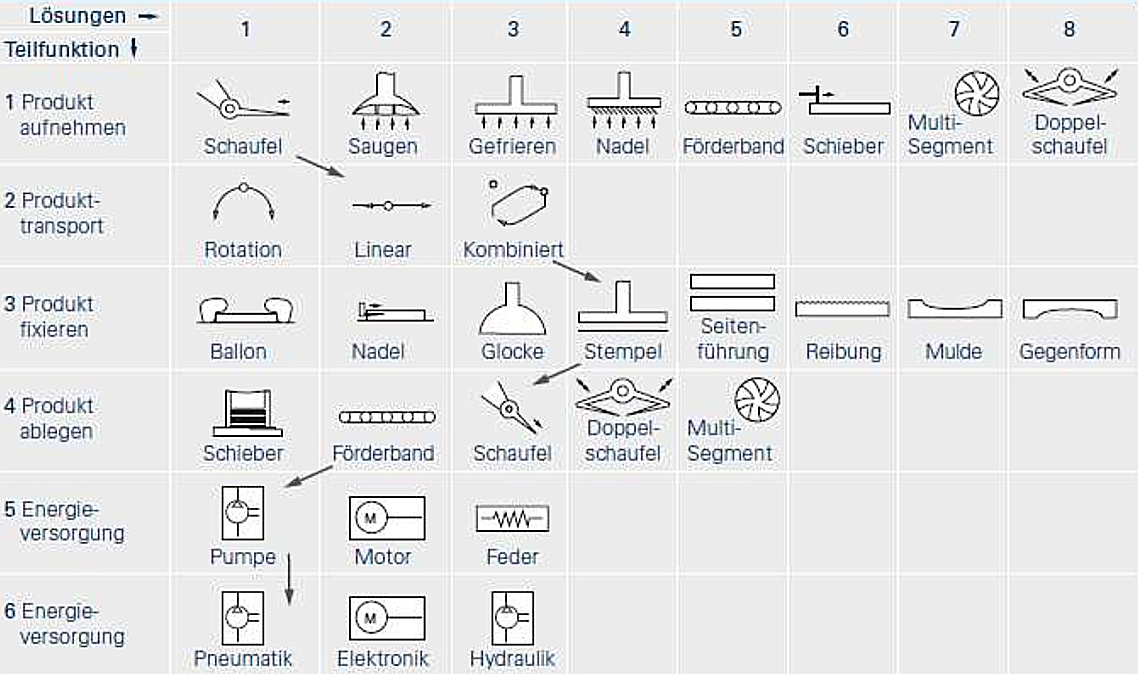
\includegraphics[width=0.9\linewidth]{./bilder/GreiferLosung}
\end{minipage}
\begin{minipage}{0.5\linewidth}
    \subsection{Last}
    \begin{itemize}
        \item Effektrolast
        \begin{itemize}
            \item Last die \textbf{als} Werkzeug oder Greifer angebracht ist
        \end{itemize}
        \item Nutzlast
        \begin{itemize}
            \item Last, welche zusätzlich zur Effektorlast bewegt werden kann ohne das daraus Einschränkungen in Geschwindigkeit, Beschleunigung oder Genauigkeit entstehen
        \end{itemize}
    \end{itemize}
\end{minipage}
\begin{minipage}{0.5\linewidth}
    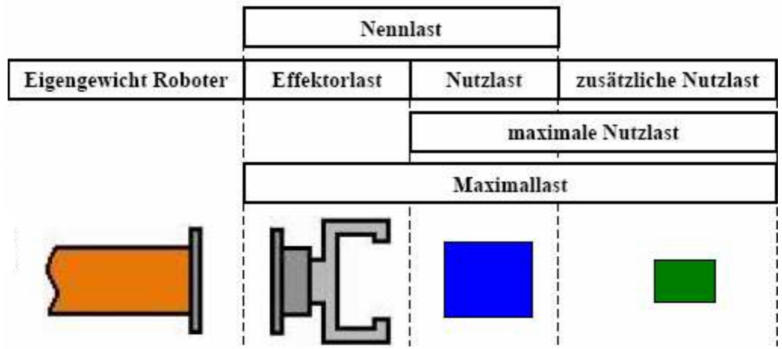
\includegraphics[width=\linewidth]{./bilder/RobLast}
\end{minipage}
\clearpage
\subsubsection{Nutzlast bei verschiedenen Roboterkinematiken}
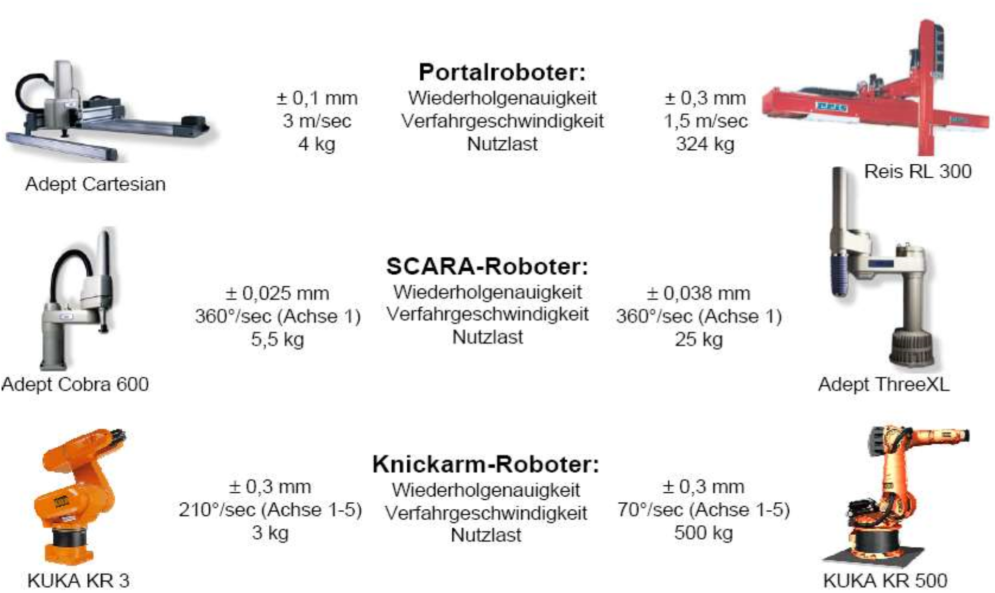
\includegraphics[width=1\linewidth]{./bilder/RobLastdiffKin}
\enlargethispage{3\baselineskip}
\subsection{Greifer}
\raisebox{-1\height}{
\begin{minipage}{0.5\linewidth}  
    \subsubsection{Halteprinzipien}
    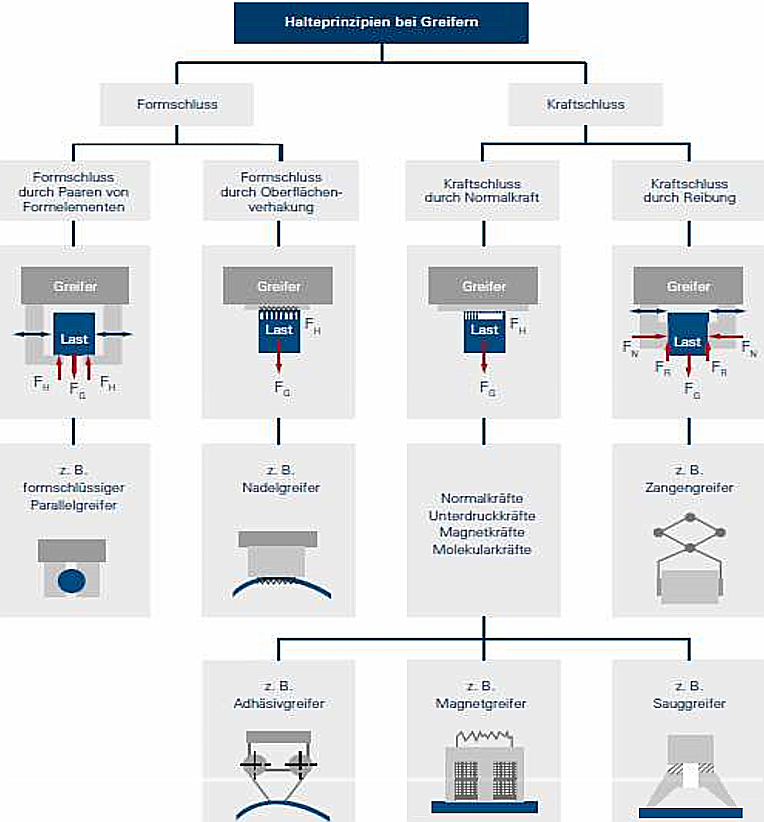
\includegraphics[width=\linewidth]{./bilder/HalteprinzGreif}
\end{minipage}}
\begin{minipage}[t]{0.5\linewidth}
    \subsubsection{Gliederung nach Wirkprinzip}
    \begin{tabular}{p{0.4\linewidth} p{0.6\linewidth}}
        \textbf{Mechanischer Greifer}&
            Zangen-, Klemm-, Gelenkfingerger-, Verhakenden Greifer (Klettgreifer, Nadelgreifer)\\
        \textbf{Pneumatische Greifer}&
            Überdruckgreifer: Loch-, Zypfen, Schrumpfring-,Luftstrahl-,Membrangreifer\\
        \textbf{Pneumostatische Pneumodynamische}&
            Unterdruckgreifer: Vakuumsauger,Haftsauger,Luftstromgreifer\\
        \textbf{Elektrische Greifer}&
            Magnetgreifer, Elektrostatische Greifer\\
        \textbf{Adhäsove Greifer}&
            Kapillar-, Gefrier-, Klebstoffgreifer\\
    \end{tabular}
\end{minipage}
\clearpage

\begin{multicols}{2}
    \subsubsection{Anforderungen}
    \begin{itemize}
        \item Greifkraft
        \item Baugrösse
        \begin{itemize}
            \item Unnötoge Störkonturen vermeiden
            \item möglichst klein/kompakt
        \end{itemize}
        \item Anschlussmöglichkeiten
        \begin{itemize}
            \item Fixiermöglichkeit für wiederholgenauen Austausch
        \end{itemize}
        \item Schnittstelle Greifer
        \begin{itemize}
            \item Exakte, spielfreie, verdrehsichere Aufnahme
            \item Schlupffreie Übertragung der Kräfte und Momente
            \item Verlustfreie Übertragung (pneu.,el.,hyd. Energie) auf Antrieb
        \end{itemize}
        \item Greifergewicht
        \begin{itemize}
            \item EInfluss auf Traglast
        \end{itemize}
        \item Greifkraftsicherung
        \begin{itemize}
            \item Bei Energieausfall muss die Spannkraft des Greifers erhalten bleiben und Handhabungsobjekt sichern
        \end{itemize}
        \item Greiferlebensdauer
        \begin{itemize}
            \item Einflussfaktoren: Lebensdrauer der Fertigungstoleranz, Fingerlänge, Kühlschmiermittel, Taktzahlen, Wartung, äussere Kräfte, Temperatur, kinemat. Wirkprinzip
        \end{itemize}
        \item Öffnungs- und Schliesszeiten
        \item Wartungsarm
        \item Schmutzunempfindlich    
    \end{itemize}
\end{multicols}
\begin{minipage}{0.5\linewidth}
    \subsection{Sauggreifer}
    \begin{itemize}
        \item Kraftschluss wird durch unterschiedliche Druckverhältnisse erzeugt
        \item Arten/Prinzip
        \begin{itemize}
            \item Vakuumsauger $\rightarrow$ Vakuumpumpe
            \item Luftstromsauger $\rightarrow$ Venturidüse
            \item Haftsauger $\rightarrow$ Saugnapf anpressen
        \end{itemize}
        \item Einsatzgebiete
        \begin{itemize}
            \item Haftsauger $\rightarrow$ glatte, luftundurchlässige Werkstückoberflächen
            \item Vakuum- Luftstromsauger $\rightarrow$ weniger glatte bis raue und poröse Oberflächen
        \end{itemize}
        \item Haltekraft
        \begin{itemize}
            \item[] $ F_h=A\cdot p_u$
            \item[] $ p_u= \frac{m\cdot g}{A \cdot \eta}$
            \item[] $F_h$= Haltekraft [N],$A$= Fläche [$cm^2$]
            \item[] $p_u$=Unterdruck [$N/cm^2$], $\eta$=dyn. Viscosität [$kg/(m\cdot s)$]
            \item[] Haltrekraft mal Sicherheitsfaktor 2
        \end{itemize}
    \end{itemize}
\end{minipage}
\begin{minipage}{0.5\linewidth}
    \subsection{Mechanische Greifer}
        \begin{itemize}
            \item Einfinger-, Zweifinger- oder Mehrfinger Ausführung
            \item Starr-, Starr-gelenkiger- oder elastischer Ausführung
            \item Antrieb erfolgt mechanisch, pneumatisch oder elektrisch
        \end{itemize}
    \begin{center}
        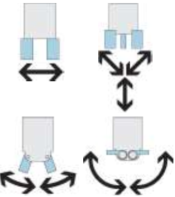
\includegraphics[width=0.3\linewidth]{./bilder/GreiferAusfurung}
    \end{center}
    \begin{minipage}{0.49\linewidth}
        \textbf{Greifkraft beim Abheben}\newline
        \null\qquad$F_G=\frac{m \cdot (g + a)}{\mu \cdot a} $\newline
        \textbf{Greifkraft beim Querhub}\newline
         \null\qquad$F_G=\frac{m \cdot g \dot S}{\mu \cdot n} + m \cdot a $
    \end{minipage}
    \begin{minipage}{0.5\linewidth}
    $n$: Anz. Greifbacken\newline
    $\mu$: Reibkoeff. Greifer zu WS\newline
    $m$: Masse des WS [kg]\newline
    $a$: Beschleunigung der dyn. Bewegung [$m/s^2$]\newline
    $S$: Sicherheitsfaktor\newline
    $g$: Erdbeschleunigung 9.81[$m/s^2$]
    \end{minipage}
\end{minipage}

\begin{minipage}{0.7\linewidth}
    \subsubsection{Auswahl}
     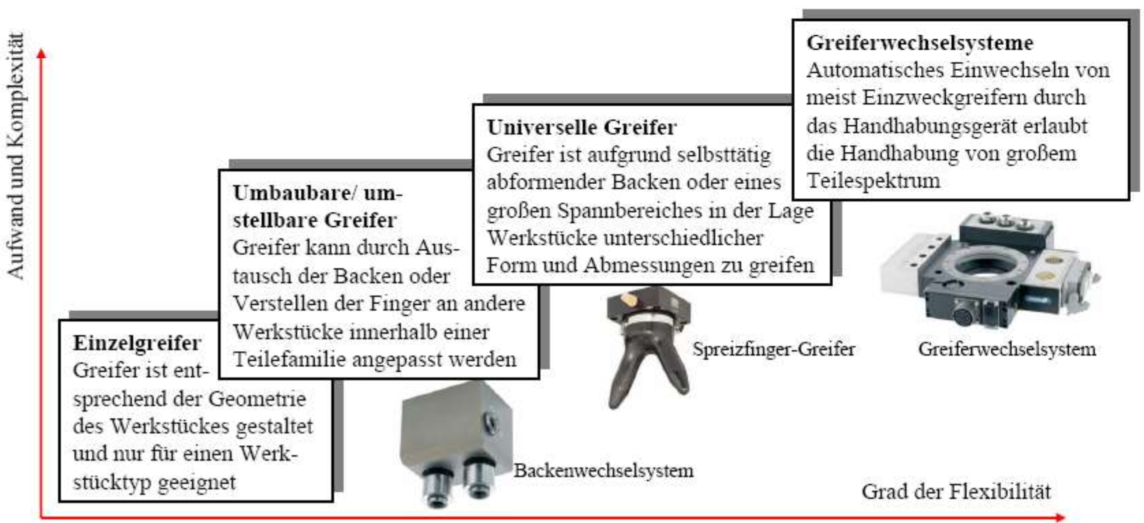
\includegraphics[width=\linewidth]{./bilder/GreiferAuswahl}
\end{minipage}
\clearpage

\subsection{Sensorik}
\begin{minipage}{0.5\linewidth}
    \subsubsection{Ziele}
   \begin{itemize}
       \item Abstandserkennung zwischen Obj. und Greifer
       \item Objektkontakt am Greifer
       \item Objekt im Greifer?
       \item Objekt korrekt gegriffen?
       \item rutscht das Objet vom Greifer?
   \end{itemize}
\end{minipage}
\begin{minipage}{0.5\linewidth}
    \subsubsection{Typische Sensoren}
    \begin{itemize}
        \item Videokameras (oft s/w)
        \item Ultraschallsensor (Rechtwinklig)
        \item Laser oder IR- Distanzsensoren
        \item Induktive Sensoren (kleine Distanzen)
        \item Lichtschranke oder Induktive Senosoren
        \item Kraft-/Momentsensoren am Greifer
    \end{itemize}
\end{minipage}
 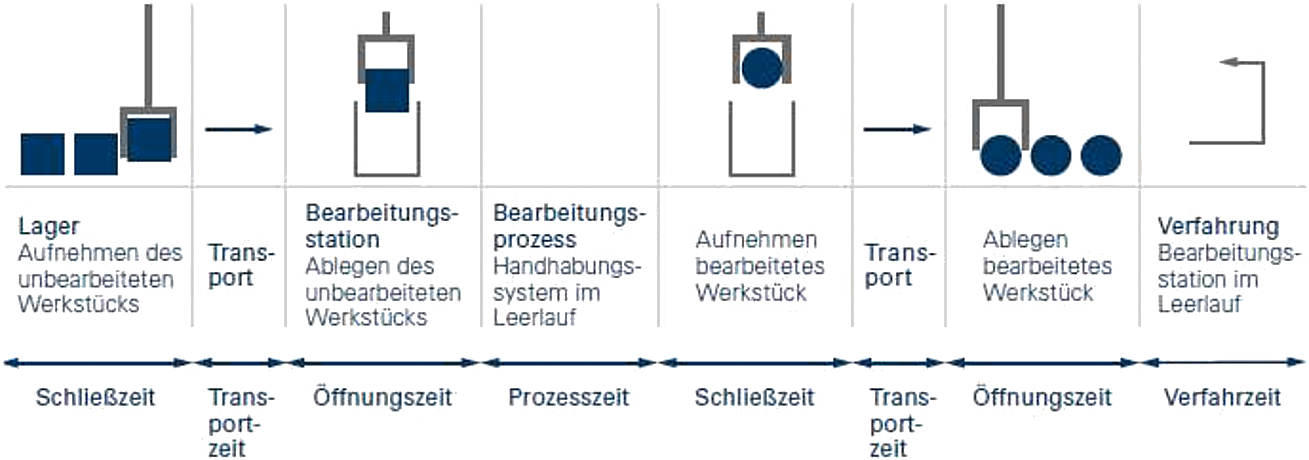
\includegraphics[width=\linewidth]{./bilder/GreiferZyklus}
 
 \subsubsection{Kamerasysteme}
 \begin{tabular}{p{5cm}p{6cm}p{6cm}}
    \textbf{Stationäre Kammera}\newline
    Transformation vom Kamera-KS ins Basis-KS&
    \begin{itemize}
        \item[+] Ist keine Last für den Roboter
    \end{itemize}
    &
        \begin{itemize}
        \item[-] Messgenauigkeit begrenzt, da die Kamera relativ weit weg vom Objekt ist.
        \item[-] Roboter evt. im Blickfeld
        \item[-] Vermessung des Kamerasichtfeldes
    \end{itemize}\\
    \textbf{Bewegte Kamera}\newline
    Transformation vom Kamera-KS ins Werkzeug-KS&
    \begin{itemize}
        \item[+] Gute Messgenauigkeit, da nah am Objekt
        \item[+] Kein grosses Sichtfeld nötig
        \item[+] Keine Tragkonstrukiton für die Kamerafixierung notwendig.
    \end{itemize}&
    \begin{itemize}
        \item[-] Werkzeug evt. im Bild
        \item[-] Kamera kann durch Kollision beschödigt werden.
        \item[-] Kameragewicht am Werkzeug reduziert Traglast.
    \end{itemize}\\
 \end{tabular}

 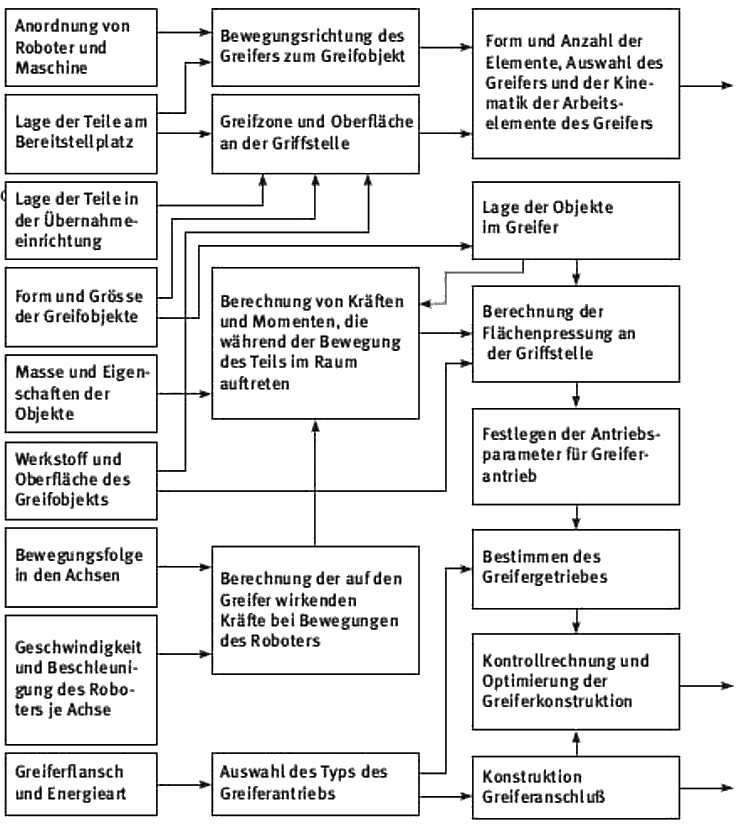
\includegraphics[width=0.7\linewidth]{./bilder/GreiferProject}